\documentclass[]{article}
\usepackage{lmodern}
\usepackage{amssymb,amsmath}
\usepackage{ifxetex,ifluatex}
\usepackage{fixltx2e} % provides \textsubscript
\ifnum 0\ifxetex 1\fi\ifluatex 1\fi=0 % if pdftex
  \usepackage[T1]{fontenc}
  \usepackage[utf8]{inputenc}
\else % if luatex or xelatex
  \ifxetex
    \usepackage{mathspec}
  \else
    \usepackage{fontspec}
  \fi
  \defaultfontfeatures{Ligatures=TeX,Scale=MatchLowercase}
\fi
% use upquote if available, for straight quotes in verbatim environments
\IfFileExists{upquote.sty}{\usepackage{upquote}}{}
% use microtype if available
\IfFileExists{microtype.sty}{%
\usepackage{microtype}
\UseMicrotypeSet[protrusion]{basicmath} % disable protrusion for tt fonts
}{}
\usepackage[margin=1in]{geometry}
\usepackage{hyperref}
\hypersetup{unicode=true,
            pdftitle={Reporte 3 MSE},
            pdfauthor={Marcos Arteaga , Claudio Gatica},
            pdfborder={0 0 0},
            breaklinks=true}
\urlstyle{same}  % don't use monospace font for urls
\usepackage{graphicx,grffile}
\makeatletter
\def\maxwidth{\ifdim\Gin@nat@width>\linewidth\linewidth\else\Gin@nat@width\fi}
\def\maxheight{\ifdim\Gin@nat@height>\textheight\textheight\else\Gin@nat@height\fi}
\makeatother
% Scale images if necessary, so that they will not overflow the page
% margins by default, and it is still possible to overwrite the defaults
% using explicit options in \includegraphics[width, height, ...]{}
\setkeys{Gin}{width=\maxwidth,height=\maxheight,keepaspectratio}
\IfFileExists{parskip.sty}{%
\usepackage{parskip}
}{% else
\setlength{\parindent}{0pt}
\setlength{\parskip}{6pt plus 2pt minus 1pt}
}
\setlength{\emergencystretch}{3em}  % prevent overfull lines
\providecommand{\tightlist}{%
  \setlength{\itemsep}{0pt}\setlength{\parskip}{0pt}}
\setcounter{secnumdepth}{0}
% Redefines (sub)paragraphs to behave more like sections
\ifx\paragraph\undefined\else
\let\oldparagraph\paragraph
\renewcommand{\paragraph}[1]{\oldparagraph{#1}\mbox{}}
\fi
\ifx\subparagraph\undefined\else
\let\oldsubparagraph\subparagraph
\renewcommand{\subparagraph}[1]{\oldsubparagraph{#1}\mbox{}}
\fi

%%% Use protect on footnotes to avoid problems with footnotes in titles
\let\rmarkdownfootnote\footnote%
\def\footnote{\protect\rmarkdownfootnote}

%%% Change title format to be more compact
\usepackage{titling}

% Create subtitle command for use in maketitle
\newcommand{\subtitle}[1]{
  \posttitle{
    \begin{center}\large#1\end{center}
    }
}

\setlength{\droptitle}{-2em}
  \title{Reporte 3 MSE}
  \pretitle{\vspace{\droptitle}\centering\huge}
  \posttitle{\par}
  \author{Marcos Arteaga , Claudio Gatica}
  \preauthor{\centering\large\emph}
  \postauthor{\par}
  \predate{\centering\large\emph}
  \postdate{\par}
  \date{28 septiembre 2017}


\begin{document}
\maketitle

\section{Resumen}\label{resumen}

Se realiza un análisis del reclutamiento de sardina común y anchoveta.
Esto implica revisión de estimaciones, patrones temporales, relación
entre especies y expresión de reclutamiento.

\section{Actividades}\label{actividades}

\begin{enumerate}
\def\labelenumi{\arabic{enumi}.}
\item
  Revisión de expresiones de reclutamiento modelos de estimación, y
  modelo operativo.
\item
  Análisis de salidas de modelos, confección tablas, gráficos y
  exploración de patrones (i.e.~alternancia).
\end{enumerate}

\emph{Modelo estimación} \textbf{codificación admb}

mean\_log\_rec1 18

mean\_log\_rec 18

init\_bounded\_dev\_vector rec\_dev(styr,endyr,-20,20,ph\_recdev)

for (int j=2;j\textless{}=nages;j++) \{natage(styr,j)=
mfexp(log\_Nini+log\_dev\_ini(j))+0.5*square(sigr);\}

\textbf{Formulación} \emph{Abundancia inicial} \[
N_{a,1}=\left(R_{0}e^{-\sum_{a} aZ_{a,t=1}}\right)e^{\epsilon_a+0.5\sigma^2_R} 
\]

Luego, la totalidad de expresiones del modelo de estimación estan en
reporte:

archivo (Modelo\_estimacion.pdf)

\subsection{Plots de reclutamiento}\label{plots-de-reclutamiento}

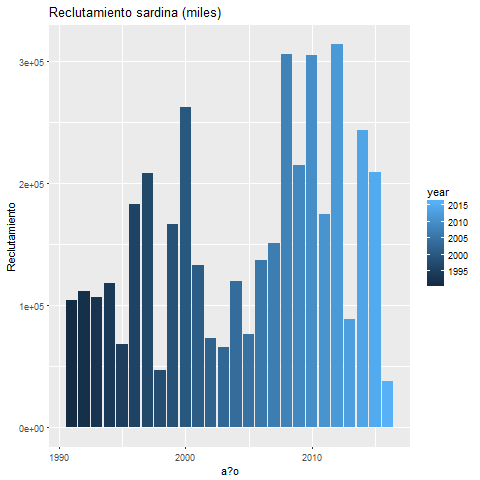
\includegraphics[width=0.50000\textwidth]{Figuras/1.png}
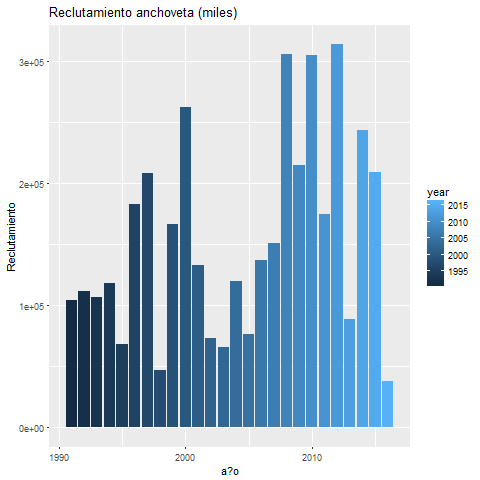
\includegraphics[width=0.50000\textwidth]{Figuras/2.png}

\newpage

Reclutamiento sardina común % latex table generated in R 3.2.2 by xtable 1.8-2 package
% Thu Sep 28 14:42:42 2017
\begin{table}[ht]
\centering
\caption{reclutamiento sardina comun} 
\label{Tabla1}
\begin{tabular}{rrr}
  \hline
 & year & Reclutas \\ 
  \hline
1 & 1991.00 & 101570.00 \\ 
  2 & 1992.00 & 183197.00 \\ 
  3 & 1993.00 & 124841.00 \\ 
  4 & 1994.00 & 114269.00 \\ 
  5 & 1995.00 & 160851.00 \\ 
  6 & 1996.00 & 126842.00 \\ 
  7 & 1997.00 & 249425.00 \\ 
  8 & 1998.00 & 165802.00 \\ 
  9 & 1999.00 & 185705.00 \\ 
  10 & 2000.00 & 164979.00 \\ 
  11 & 2001.00 & 122417.00 \\ 
  12 & 2002.00 & 166284.00 \\ 
  13 & 2003.00 & 210197.00 \\ 
  14 & 2004.00 & 256443.00 \\ 
  15 & 2005.00 & 156292.00 \\ 
  16 & 2006.00 & 193517.00 \\ 
  17 & 2007.00 & 211696.00 \\ 
  18 & 2008.00 & 82104.20 \\ 
  19 & 2009.00 & 55117.30 \\ 
  20 & 2010.00 & 29524.90 \\ 
  21 & 2011.00 & 20472.00 \\ 
  22 & 2012.00 & 16268.00 \\ 
  23 & 2013.00 & 28805.50 \\ 
  24 & 2014.00 & 33607.40 \\ 
  25 & 2015.00 & 30716.90 \\ 
  26 & 2016.00 & 122987.00 \\ 
   \hline
\end{tabular}
\end{table}
 \newpage
Reclutamiento anchoveta % latex table generated in R 3.2.2 by xtable 1.8-2 package
% Thu Sep 28 14:42:42 2017
\begin{table}[ht]
\centering
\begin{tabular}{rrr}
  \hline
 & year & Reclutas \\ 
  \hline
1 & 1991.00 & 104085.00 \\ 
  2 & 1992.00 & 111188.00 \\ 
  3 & 1993.00 & 106993.00 \\ 
  4 & 1994.00 & 118322.00 \\ 
  5 & 1995.00 & 68043.10 \\ 
  6 & 1996.00 & 182563.00 \\ 
  7 & 1997.00 & 207756.00 \\ 
  8 & 1998.00 & 46623.70 \\ 
  9 & 1999.00 & 166448.00 \\ 
  10 & 2000.00 & 262395.00 \\ 
  11 & 2001.00 & 133245.00 \\ 
  12 & 2002.00 & 73424.10 \\ 
  13 & 2003.00 & 65567.70 \\ 
  14 & 2004.00 & 119688.00 \\ 
  15 & 2005.00 & 76186.50 \\ 
  16 & 2006.00 & 136547.00 \\ 
  17 & 2007.00 & 151073.00 \\ 
  18 & 2008.00 & 305358.00 \\ 
  19 & 2009.00 & 214987.00 \\ 
  20 & 2010.00 & 304877.00 \\ 
  21 & 2011.00 & 174389.00 \\ 
  22 & 2012.00 & 313814.00 \\ 
  23 & 2013.00 & 88624.40 \\ 
  24 & 2014.00 & 243506.00 \\ 
  25 & 2015.00 & 208861.00 \\ 
  26 & 2016.00 & 37944.20 \\ 
   \hline
\end{tabular}
\end{table}



\end{document}
